\chapter{Models@Runtime for the IoT}
\label{ch:MARContiki}
%Introduction
%Taking into account the distributed nature of the IoT environment, we can observe that deployment of new functions and updates for bug fixing is a very challenging task.
%Thus, designing a tool able to provide such capacities in this constrained context raises several scientific challenges.
%All the following challenges are related to the limited resources of these nodes and the particular topology of the network that interconnect them.
%We address the problem of enabling the deployment of a distributed software layer and its dynamic reconfiguration over a network of nodes featuring very limited resources: memory, processing power, bandwidth communication and energy autonomy.

% limitation of SOTA
Looking at our state of the art, various techniques have been proposed to enable software updates, which were presented in table \ref{tab:deployMethods}.
As for the full kernel replacement mechanism, which can be managed by an automatic tool \cite{hui2004dynamic}, the excessive amount of power needed by this approach does not seem appropriated for a highly dynamic infrastructure such as the IoT.
The approaches making use of virtual machines were already analysed and it was found that they are not suitable for long-living applications \cite{oliver2014reprogramming}.
Even if some component models  \cite{mottola2008figaro},  \cite{taherkordi2013optimizing} were proposed to provide an abstraction layer for the life-cycle maintenance, it results in a very complex programming model and routing protocols to distribute components, in addition to a finely tuned memory manager for specific platforms and hardware architectures, which reduces scalability.
Thus, the lack of a deployment manager which leverages kernel modularization using relocation mechanisms, which seems the best way to provide new features and updates, motivates our research to find an automatic and scalable approach to provide such a manager.

In this chapter, we describe the main challenges while designing a new middleware dedicated to IoT devices, in order to enable the management of software deployment and the dynamic reconfiguration of IoT systems.
Indeed, our middleware is inspired from the Component Based Systems and the model@runtime paradigm which have been already described in the previous chapter.
%%As presented in chapter \ref{ch:IoT}, Internet of Things systems are typically formed by a myriad of many small interconnected devices.
%%This underlying hardware infrastructure raises new challenges in the way we administrate the software layer of these systems.
%%Indeed, the limited computing power and battery life of each node combined with the very distributed nature of these systems, greatly adds complexity to distributed software layer management.


%%The capacity of dynamically deploying and reconfiguring the software layer on the IoT is a crucial feature.

%%Therefore, a simple adaptation of an existing implementation for deployment and reconfiguration in distributed systems would not fit on a typical IoT device.
%%Indeed, the very scarce resources limits the use of complex approaches \textit{"as is"}, as it was already described in section \ref{sec:dynamicDeploymentDAS}

%%Indeed, the previously studied models@runtime approach, and more specifically, the Kevoree approach, provides a way to manage the application layer for distributed systems.
%%As stated in section \ref{sec:distDeployment}, the high resemblance between distributed systems and the IoT, makes the use of such approach a viable solution.
%%However, the huge differences in computing capacity and energy autonomy between the nodes involved in both scenarios make the implementation of this approach very challenging.
%%Thus, a direct mapping of Kevoree (the meta-model and its model manipulation tools) cannot be foreseen.

%%Moreover, our proposition is based on an existing implementation of the paradigm of models@runtime which has been adapted to fit IoT devices constraints.

%%Moreover, the implementation of this middleware follows the directions of the existing Kevoree meta-model depicted in \todo{annex or figure?}, which has been adapted to fit IoT devices constraints. 
%As a matter of fact, our evaluation of these constraints was conducted on several hardware platforms typical of the IoT, in order to establish a reference for the minimum requirements to run such a middleware.
%%Once an initial research on these IoT platforms was conducted, the proposition of a new one was necessary, since the minimal requirements were not met by the commercially available platforms at that time.
%%Such platform was an essential part to evaluate our first implementation, and was used to establish the minimum requirements of an execution environment.
%%Finally, we have conducted the evaluation of our approach on an Internet of Things testbed \cite{Fleury15iotlab} recently available for experimentation.
%%Our results demonstrates the feasibility of providing a model@runtime middleware for these systems, which can be executed in platforms meeting the requirements already established.
%%This chapter is concluded by the obtained results on the FIT IoT-Lab testbed, which show the limits of our first approach.
\section{IoT specific requirements for model@runtime}
As mentioned in the previous chapter, the model@runtime approach has been proposed and designed for distributed systems where nodes are powerful computers interconnected through a very high-speed network. 
Some inherent characteristics of this approach were thus designed without taking into consideration the very specific and constrained nature of IoT systems.
In this section, we present the specific characteristics of IoT systems which make them incompatible with the current design of Model@Runtime, and we elicit a set of requirements to design a model@runtime approach for IoT systems.

Compared to a classical distributed system, an IoT system mainly differs through the three following characteristics:
\begin{itemize}
	\item an \textbf{energy constraint}: most nodes included in an IoT system are battery powered with limited capacity. This particular way of powering the computing nodes has a direct impact on the development of software. Indeed, if the software running on those systems have not been designed with the energy constraint in mind, it will drastically reduce the life time of the system.
	\item a \textbf{very limited computing and memory resource}: most nodes included in an IoT system presents a very limited amount of computing and memory resources compared to a more classical computing node. These resource constraints have an impact on software development since classical algorithm and design may not fit into such constraints.
	\item a \textbf{multi-hop routing infrastructure}: in an IoT system, most nodes are interconnected through a multi-hop routing infrastructure. This specific way of routing packets through other nodes in the network directly impact the way of designing inter nodes communication since fulfilling any specific network communication may drain energy and computational resources from several nodes in the network.
\end{itemize}

Therefore, designing a specific model@runtime approach for IoT system will require to cope with these three main characteristics which differs from classical distributed systems. 
Typically, a model@runtime approach for distributed system is designed with two main components:
\begin{itemize}
	\item a \textbf{model}: which represents the current state of the whole distributed system. This model typically represent three layers : (i) \textbf{the hardware level} with all nodes included in the system; (ii) \textbf{the network level} with all communication path between the nodes, and (iii) \textbf{the software level} with all software components, their configurations and their communications paths. This model is used as the corner stone of the approach to deploy and perform dynamic evolution of the software system.
	\item a \textbf{software agent}: running on all nodes. This software agent is in charge of all activities to transform this declarative model into a running system. These activities include model interpretation (loading, comparison, and so on), software component downloading, and dynamic software loading. All software agents in the system are independent and performs independently the specific tasks needed on each node.
\end{itemize}

In an IoT system, the software agent has to be redesigned and implemented in a different way to take more carefully into account the three inherent characteristics described above.
The model has to remain the same conceptually, in order to interoperate with hybrid systems which includes IoT nodes together with computing nodes with less limitation of computing power. 
We divided the problem of designing a model@runtime approach for IoT into the following two main challenges:
\begin{itemize}
	\item the \textbf{intra-node challenge}. This challenge is related to designing the software agent part together with a typical IoT node in order to fit all activities related to local model interpretation and dynamic software loading into the resource constraints IoT node. This challenge also relates to the evaluation and minimization of the performance and energy overhead of the model@runtime approach. 
	\item the \textbf{inter-node challenge}. This challenge is related to the design of new communication schemes to take into account the underlying routing topology, in order to minimize the energy consumption of the required model@runtime communication. This includes in particular a communication scheme to minimize the energy consumption related to software component downloading and distribution.
\end{itemize}

\section{Kevoree for the IoT}
\label{sec:kevAndIoT}
%Dans cette section il faut reprendre les challenges dont je viens de parler dans le 4.1 et les détaillé par rapport aux différentes activités dans Kevoree. Montrer celles qui sont vraiment obligatoire etc et comment on va s'occuper de tout ca dans le contexte de Kevoree. Le but est bien de fournir un exemple plus complet et plus précis afin que le lecteur comprenne très concrètement le problème addressé dans la thèse et la grande idée de la solution.
Focusing on our first challenge, the intra-node case, we aim to develop a software agent able to provide a set of tools to leverage the models@runtime advantages and properties, in order to provide an automatic platform for IoT software deployment and maintenance.
This section will present the design of such an agent, taking into account the previously mentioned characteristics.

One of the models@runtime approach implementations already discussed was the Kevoree framework.
As presented in section \ref{sec:MAR_overview}, the base of this framework is the Kevoree meta-model, which was designed to follow a distributed architecture and also offers a minimalistic component model.
Indeed, the implementation and design of Kevoree did not take into account any restriction on the underlying system, thus relying on high memory and storage capabilities with fast processing features.
Thus, we cannot envision the direct mapping of this implementation on very constrained nodes such as IoT nodes.

However, some of the Kevoree activities are interesting for their use on a distributed environment such as the IoT.
Indeed, Kevoree is able to perform reconfiguration and deployment tasks, which are the main functionalities we are searching for.
To be precise, we are interested on the following features:

\begin{itemize}
	\item \textbf{The meta-model to represent the whole distributed system.} The representation proposed by Kevoree through the meta-model is very close to our IoT environment, since it focuses on independent nodes and provides abstractions for the communication means, which is the main activity of an IoT node.
	\item \textbf{Principles for model manipulation.} Several tools are needed while changes on the system are reflected on the model. It is then needed to change parameters, add or remove components, check for changes between old and new models and so on. Thus, tools like model serializer/deserializer, model comparing, and model visitors, are essential for a functional Kevoree implementation.
	\item \textbf{Kevoree editor} A web editor is available for model checking/editing. This is very useful while triggering adaptations by hand.
\end{itemize}
\begin{figure}[]
	\centering
	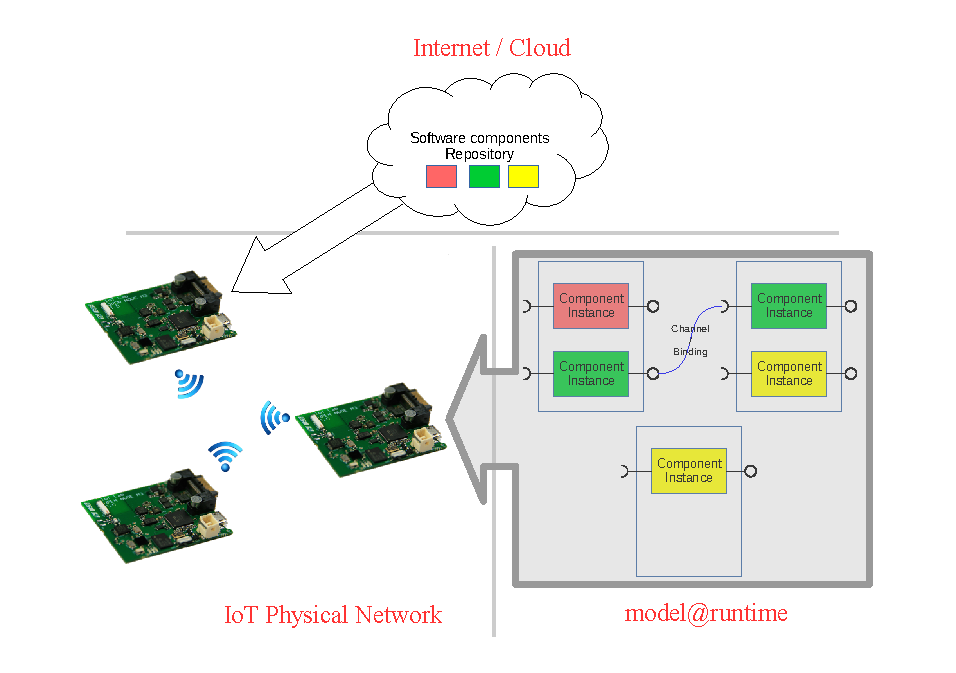
\includegraphics[width=1\columnwidth]{chapters/modelsAtRuntimeContiki.images/MAR_IOT.pdf}
	\caption{A M@R representation for IoT devices}
	\label{fig:MAR_IOT}
\end{figure}
Our goal is then to provide a middleware that will be present on each node of the IoT system, and will take care of the various tasks imposed by the model@runtime paradigm.
In figure \ref{fig:MAR_IOT}, we can see a representation in which three IoT nodes are part of a small network.
This example shows how the model is present on the three nodes, each node having the knowledge about three available components on the repository, the instances present in the other two nodes and a binding through a channel between two components of different nodes.
Moreover, any change of this configuration should be reflected on the model, followed by the dissemination of these changes to the other nodes, and vice-versa, any change on the model will affect the actual node.
Figure \ref{fig:MAR_modelListenerIoT} describes the actions taken when a reconfiguration or adaptation is triggered.

%\begin{figure}[]
%	\centering
%	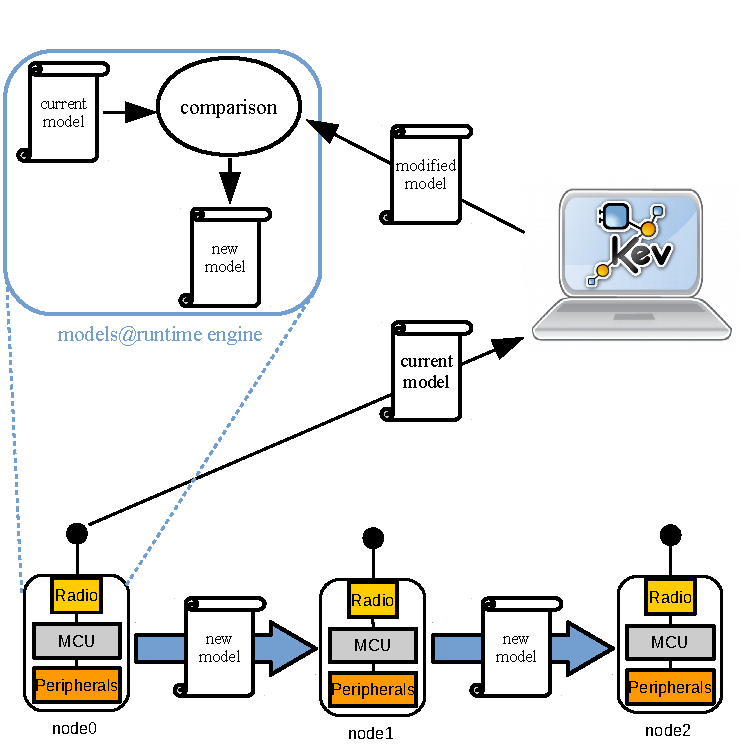
\includegraphics[width=1\columnwidth]{chapters/modelsAtRuntimeContiki.images/reconfigMAR.pdf}
%	\caption{Reconfiguration through a M@R}
%	\label{fig:MAR_reconfig}
%\end{figure}

%Following the directions presented above, an implementation of this approach on IoT nodes has been conducted, which should be able to have a similar model representation in memory and to enact the adaptation and reconfiguration process on each node.
%As we stated before, the exact implementation of the Kevoree M@R approach using the current tools is not feasible, due to the IoT node's constraints.
Thus, we need to leverage only the previously described mechanisms provided by this approach, and adapt the selected features to address the node's hardware constraints.
The next Subsection will take into consideration the minimal requirements towards the design of a new M@R implementation for IoT nodes, inspired from the Kevoree approach.
%It is also important to offer a similar behaviour and interoperability with the other Kevoree implementations.

%Thus, a first challenge lies in the implementation of such meta-model meeting the programming language and memory constraints.

\subsection{Minimal Kevoree properties needed on the IoT}
\label{subsec:minKevProp}
As already discussed in section \ref{sec:MAR_overview}, the Kevoree meta-model can be easily transformed into Java code using a modelling framework.
However, in our case this approach cannot be used.
This is due to two reasons: first, we cannot use high-level languages such as Java and second, we are limited to the C language which can be compiled for the IoT node's architecture already presented in \ref{subsec:smartObjects}.
Moreover, meta-models follow very often an object-oriented approach, which is not defined for procedural languages such as C.
Thus, a direct transformation taking into account this constraints is not worth considering.
However, a similar approach for code generation and modelling tools can be proposed to meet the requirements of a model@runtime approach.
Indeed, the Kevoree Modelling Framework \cite{fouquet2012eclipse} can be adapted to support the generation of C code, in order to provide a fully Kevoree-like middleware for IoT devices.
Even so, the efforts to adapt such a framework raise more and different challenges which are out of the scope for this thesis.
Since our goal is, first of all, to investigate the limits of an IoT node in terms of memory, a manual implementation (transformation) of the meta-model and its modelling tools is then needed, by adapting the concepts to the limited resources of the node.
Indeed, this allows a rapid prototype which can be finely tuned to meet the memory constraints present in IoT devices, in contrast to a more generic code generation approach.

On the typical implementation of Kevoree, a \textit{core} application is embedded in every node. 
This application provides to each system element (node, component, communication channel, groups) an access to the current model, allowing to submit new configurations through new models.
If this \textit{Kevoree Core} receives a new model, it is in charge of the following actions:

\begin{itemize}
	\item \textbf{Model validation.} Verify if the serialized model actually corresponds to a valid Kevoree model, by parsing it and proceeding to deserialization.
	\item \textbf{Adaptation planning.} Once the model is deserialized and loaded in memory a model comparison is performed. A list of differences is then generated, describing the actual adaptations to be performed, which may contain adding/removing components and modifications to parameters (reconfiguration).
	\item \textbf{Adaptations execution.} Following the adaptation plan, the adaptations (component deployment, reconfiguration) will take place, in the following order:
	\begin{enumerate}
		\item \textbf{Stop Instance}. A running instance will be stopped.
		\item \textbf{Remove Binding.} If a binding between 2 channels of a component exists, it will be removed.
		\item \textbf{Remove Instance.} A component instance will be removed.
		\item \textbf{Remove Deploy Unit.} A deploy unit will be removed.
		\item \textbf{Update Binding.} When a binding between channels exists, it will be changed to the new channels.
		\item \textbf{Update Deploy Unit.} An existing deploy unit gets replaced by a new one (most recent version).
		\item \textbf{Add Deploy Unit.} If a new deploy unit is needed, it will be downloaded and made it available for instantiation.
		\item \textbf{Add Instance.} An instance will be created from an existing Deploy Unit.
		\item \textbf{Add Binding.} A new binding between two channels will be created.
		\item \textbf{Update Dictionary Instance.} If a dictionary entry exists for an instance, it will be updated with a new value.
		\item \textbf{Update Instance.} An existing instance will be updated with a new version.
		\item \textbf{Start Instance.} An existing instance which was stopped will be started.
	\end{enumerate}
	This order will avoid any inconsistency while performing the adaptations.
\end{itemize}

The model validation is delegated to any system element registered as a \textit{listener}.
Each component, communication channel or node can make use of an interface and be registered on the \textit{core} in charge of the model management.
Once registered, the instance is notified with regard to the different reconfiguration stages.
%For this, a \textit{listener} interface can define the following notifications:
%\begin{itemize}
%	\item \emph{preUpdate} allows to the \emph{listener}s to be notified that an update has been proposed.
%	Each \emph{listener} can then validate the proposed configuration.
%	\item \emph{preAllUpdate} allows to the \emph{listeners} to be notified that the proposed update has been validated by the set of \emph{listener}.
%	\item \emph{postUpdate} allows to the \emph{listeners} to be notified that the update has been applied.
%	Each \emph{listener} can then validate that the update does not cause a problem.
%	\item \emph{postAllUpdate} allows to the \emph{listeners} to be notified that the update which has been applied was also validated by the set of \emph{listener}s.
%	\item \emph{preRollback} allows to the \emph{listeners} to be notified that the update has failed and a rollback to the previous configuration will be carried out.
%	\item \emph{postRollback} allows to the \emph{listeners} to be notified that the rollback has been successful.
%\end{itemize}
Figure \ref{fig:MAR_modelListener} represents in a state-transition diagram the integration of \textit{listeners} with the process of a typical implementation of Kevoree.

\begin{figure}[]
	\centering
	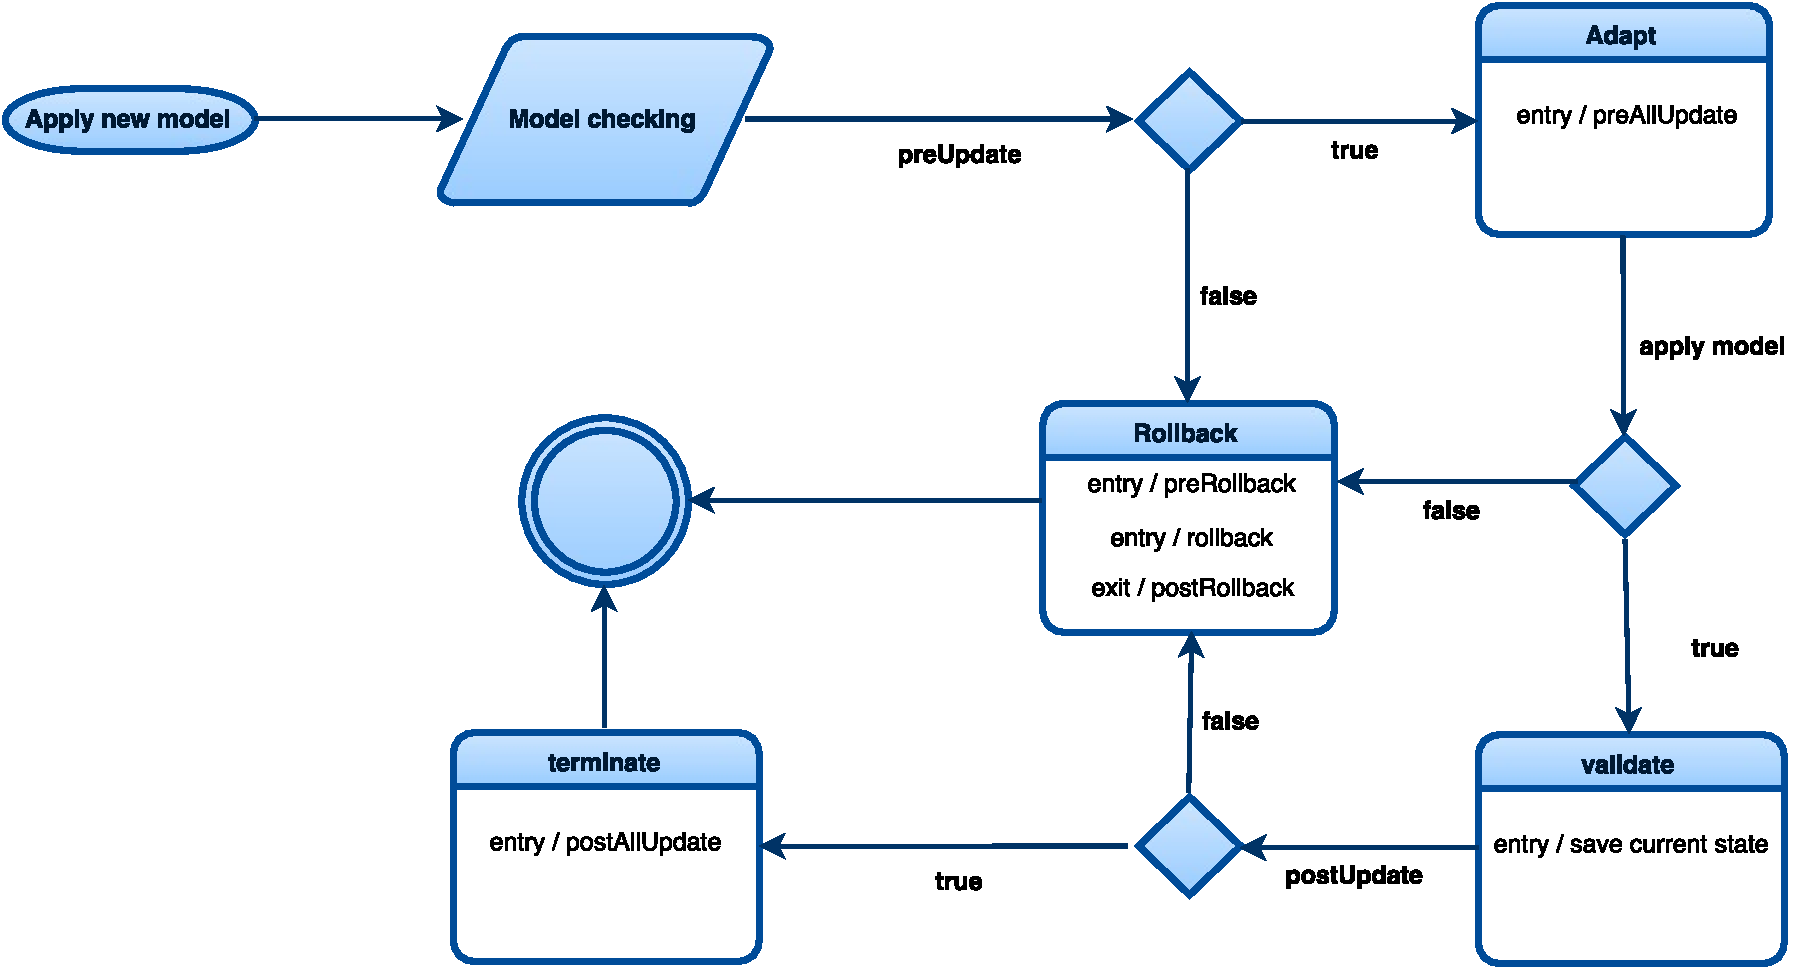
\includegraphics[width=1\columnwidth]{chapters/modelsAtRuntimeContiki.images/ModelListenerStateChart.pdf}
	\caption{State-transition diagram showing the adaptation process in a typical kevoree implementation}
	\label{fig:MAR_modelListener}
\end{figure}

In contrast, our design for IoT devices cannot follow the same algorithm.
Indeed, the model checking and rollback mechanisms require to save the entire model in memory for checking and, if something goes wrong, to bring back the previous model.
This is very memory consuming for our application, thus a typical IoT device would not be able to keep several models in RAM for the rollback mechanism.
Therefore, only a simple model checking followed by the adaptations execution has been proposed.
%Moreover, the implementation of this mechanism for all the system elements (component, communication channel, group) was not necessary for our first prototype.
%Thus, only a \textit{ModelListener} is present on our core, avoiding all the notification process, saving processing time thus energy.
Indeed, in our proposition the node is in charge of the adaptation mechanisms, since for our concerns (an IoT system) nodes are the main component and it can only execute an instance of itself.
This vision contrast with a typical Kevoree implementation, where various \textit{Kevoree Core} can run on a single machine, resulting in several nodes reflected in the model.

In figure \ref{fig:MAR_modelListenerIoT} the proposed reconfiguration algorithm is presented, which is able to modify the model retrieved from a node.  The set of adaptation stages mentioned above are then carried through a transactional manner.
%In conclusion, our proposition for a Kevoree implementation on IoT devices is conceivable, since we bring the most important features with a very low memory footprint, having only a few limitations.

\begin{figure}[]
	\centering
	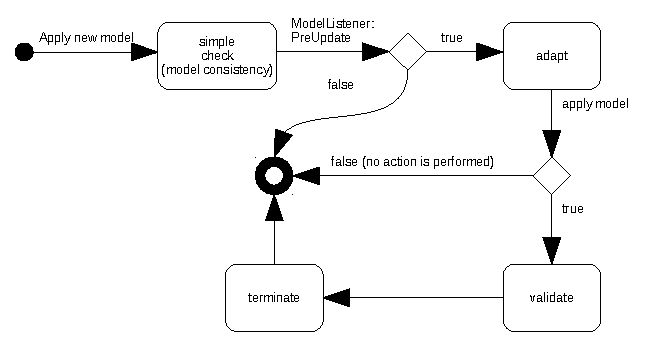
\includegraphics[width=0.85\columnwidth]{chapters/modelsAtRuntimeContiki.images/modelListenerIoT.pdf}
	\caption{State-transition diagram showing the adaptation process for IoT devices}
	\label{fig:MAR_modelListenerIoT}
\end{figure}

After describing the main design issues and challenges, we can highlight these in figure \ref{fig:MAR_Challenges}.
Indeed, a models@runtime implementation is not straightforward, and needs special attention to meet the constraints already discussed previously.
In summary, as depicted on figure \ref{fig:MAR_Challenges}, we have two aspects which result in a complete M@R implementation: the kevoree meta-model, which describes the model representation of the current system, as well as the component model, and finally the M@R engine which manipulates this model.
This engine should meet all the constraints present in an IoT device, and at the same time to provide the main functionalities to receive, compare and generate a list of found differences (traces) between the current model and a (modified) new one.
Moreover, in order to receive and send models through the network, a serializer and de-serializer is needed, using a JSON format.
In addition, a model compressor and an adaptation of Deluge \cite{hui2004dynamic} as a dissemination tool, already discussed in Subsection \ref{subsec:ImplConstraints} are also needed.
In conclusion, our middleware would be able to provide a list of needed adaptations, based on predefined adaptation primitives, such as add/remove components, change dictionary entries (parameters) and stop or start component instances.
Finally, an ordered plan to execute such adaptations is required for the actual system, which will perform the actions.
Therefore, we can now separate our approach into two different challenges: the first one, which is the meta-model and modelling engine implementations, and the second one, the system facilities development to enact the adaptations provided by the M@R engine.

\begin{figure}[]
	\centering
	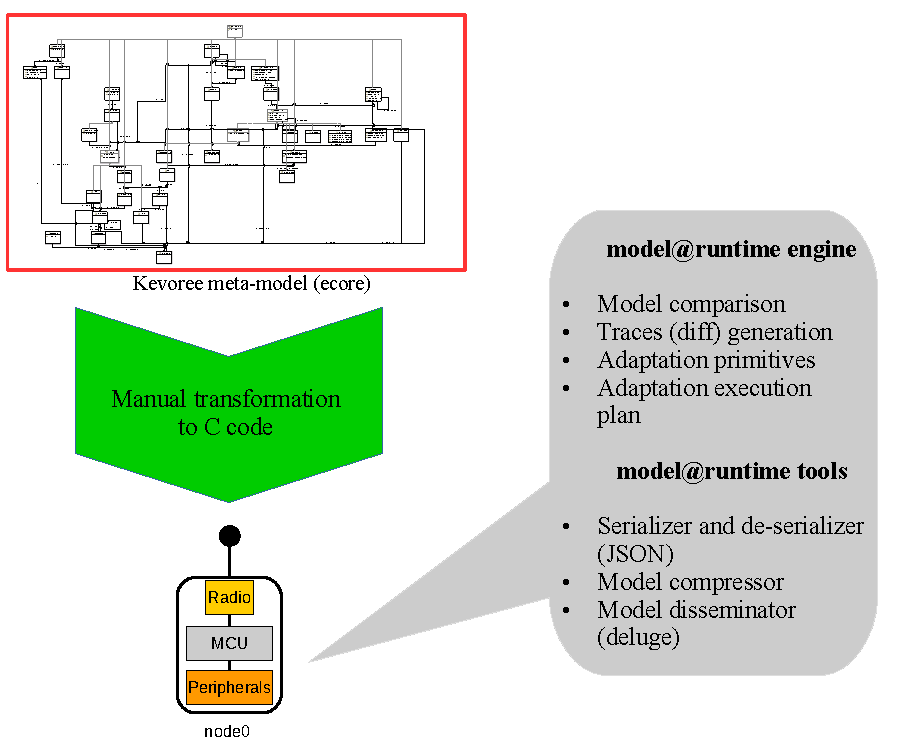
\includegraphics[width=0.85\columnwidth]{chapters/modelsAtRuntimeContiki.images/Challenges.pdf}
	\caption{The two different needs for a complete IoT models@runtime engine}
	\label{fig:MAR_Challenges}
\end{figure}

We need thus to have a clear view of the requirements while implementing such middleware, especially at the system level.
Indeed, the underlying system should provide all the needed features on which the M@R design relies.
The next Subsection will discuss these requirements in order to find an existing software platform that fits for our design.

\subsection{Kevoree software implementation requirements}
\label{sec:kevoreeRequirements}
Our middleware approach will need several features from the underlying system, in order to match with the high-level description provided by the model@runtime.
As we discussed on our state of the art in Section \ref{sec:IoTDeployment}, the most common approach used to run applications on IoT devices is bare-metal development followed by firmware flashing into the ROM memory.
Even if this method allows a fine control of the underlying hardware, the development time can be very long and difficult to debug, since abstractions are mostly done only at the hardware level, and does not come to the system level.
Moreover, since complexity grows, applications for IoT should be developed without special attention to hardware and system concerns.
Thus, the use of an IoT operating system seems to be the way to go, in order to leverage its system-level abstractions.

As presented in the state of the art, several IoT operating systems exist, but according to the needed features some of them are more convenient.
We can thus establish the requirements as following, according to OS properties:
\begin{enumerate}
	\item \textbf{Basic OS functionalities such as timers, task scheduler and Inter Process Communication (IPC).} Basic functionalities that are the core of any embedded OS.
	\item \textbf{Dynamic linker and loader, following the third approach presented in section \ref{sec:IoTDeployment}.} A dynamic linker and loader is essential to our approach, since changes in the model containing new software components will trigger the download and instantiation of an artefact, which should be linked and loaded at runtime by the underlying system.
	\item \textbf{Network stack implementing basic IP functions (TCP, UDP, HTTP, CoAP).} In order to share a model and download software artefacts, IP communication is mandatory, since the goal is to use the Internet to reach component repositories from different sources.
	\item \textbf{Persistent data handling, preferably a file system.} The method used to avoid RAM storage is to serialize the model@runtime in a file on the flash memory, usually in the JSON format. Thus, a way to store and access this JSON file for reading and writing should be provided.
	\item \textbf{Abstractions for attached devices (LEDs, sensors, actuators, etc.).} Although not mandatory, an OS usually carry basic hardware abstractions, providing an easy way to develop applications which need a physical interaction with the external world.
\end{enumerate}
In order to make a rapid functional prototype of our middleware, we will make use of the Contiki OS which, given the features presented above, seems to fit our minimal requirements.
Despite the programming model already described as a drawback, Contiki offers all the needed functionalities, as well as a wide community which collaborate very actively in the development and debug of it.
%Therefore, we use the ContikiOS \cite{dunkels2004contiki} in order to provide an efficient way to distribute components, since it allows dynamic loading of binary modules.
Moreover, Contiki includes an implementation of 6loWPAN \cite{rfc4944}, an adaptation layer for an IPv6 compressed stack, which let us assign directly an IPv6 address to the device.
This enables a ready to use IoT environment.
Afterwards, an UDP transport layer is provided, allowing a standard way to reach UDP servers to download the needed deploy units to perform system adaptations, according to the model@runtime engine.
%We use erbium's \cite{rfc7252} CoAP implementation in order to have a REST engine which is used as a main communication channel between nodes. 
Indeed, one of the most important features provided by this OS is the dynamic code loading mechanisms.
These are based on a dynamic linker and loader that use the standard ELF object file format \cite{dunkels06runtime}.

% Figure \ref{fig:MAR_modelListenerIoT} depict the state-transition diagram according to our M@R process for IoT devices.

\section{Networking aspects on IoT environments}
\label{subsec:ImplConstraints}
Regarding the \textit{inter-node} challenge, another concern while adapting the selected features of the Kevoree M@R implementation is the amount of energy needed to run it.
Indeed, an IoT device running on batteries should be able to embed this middleware without a high overhead in terms of energy consumption.
Since the most processor consuming tasks are model checking and adaptations execution, a smaller overhead is induced, compared to the traditional approach, thanks to the simplification of such process.
However, it was discussed that the most energy consuming task for an IoT device is the radio communication.
This rises new and different challenges while interconnecting our nodes running the adapted Kevoree implementation, since the traditional Kevoree implementation was done having in mind no restrictions for network usage and bandwidth, thus algorithms such as Gossip \cite{fouquet2012dissemination} were used for model dissemination.
The implementation of such a protocol in an IoT device could be very memory consuming, in addition to a high energy consumption while using the network.

Given the energy and memory constraints, a dissemination protocol adapted for IoT devices is then needed.
It results interesting that the already described Deluge protocol \cite{hui2004dynamic} seems to be a good option, since it was developed having in mind the constraints of an IoT device.
Even if it was presented as a bad choice while performing entire firmware transmissions, the model information to be shared is not as big as an entire firmware, but rather a small serialized file, thus the needed energy to disseminate a model is actually very low.

A last concern should be taken into account while performing adaptations.
We observed that the adaptation process would need to download new deploy units to be instantiated according to the new requirements, or when an update is needed.
Indeed, the traditional Kevoree approach will download all needed software artefacts from a registered repository, without any care about the network topology.
However, since the nodes on the IoT can form very different and complex network topologies (multi-hop mesh, stars), we need to analyse several strategies to reduce network traffic as much as possible.
Therefore, the need of a more complex technique to download software artefacts appears, in order to reduce the inherent energy consumption while performing this task.

%Moreover, a compression method using an association table including the most often used keywords has been proposed, reducing the model size by more than a half.
%By these means, a small file including the model is shared between all the concerned IoT nodes in the network.

%Once the set of features is built, we will proceed to a review of the current challenges in the design, and how we can address them while implementing the needed software on an actual IoT device.
%Next section will present such review.

%\subsection{Design review and challenges}
%\label{subsec:implReview}

\section{Summary}
At this point, we can highlight the main requirements and functionalities needed from a typical IoT device, in order to run a models@runtime implementation.
We can now observe that the challenges are concentrated on the internal behaviour of an IoT node, thus focusing only in providing an \textit{intra-node} implementation.
This intra-node view will guide us to put our efforts into a first proposal of the Kevoree-IoT middleware, taking into account all the design requirements exposed throughout this chapter.

It is important to notice and remember that our environment is very constrained, first in the intra-node perspective but also in the inter-node mechanisms.
Indeed, we can remember our challenges as following:

\begin{enumerate}
	\item \textbf{Intra-node challenges:} Memory, processing, storing and programming environment constraints.
	\item \textbf{Inter-node challenges:} Networking, thus communication, which impacts primary the energy consumption.
\end{enumerate}

%Figure X provides a general view of these challenges, highlighting its place on the overall research work, stating our main goals.

The next chapter will provide the implementation details of our intra-node design specifications, followed by an evaluation of the possibilities and limitations of our approach.
Since our goal is to provide a middleware that works on real platforms, our evaluations were conducted, first, on an especially designed hardware platform.
Moreover, once our first tests are analysed, we followed our research goals by testing our implementation on a large-scale testbed.
Indeed, this last evaluation will trigger the actual challenges for the inter-node needed mechanisms, which will be presented in the chapter afterwards.

%As a final consideration, the executed application contained a very minimalistic model, including only enough characteristics to manipulate such model.
%Indeed, for the next chapter, a more complete implementation of the modelling framework is proposed, resulting in a more robust middleware.
%For this reason, the size of the application can increase, and the ability to instantiate components and nodes at the model level can be decreased.
%The next chapter will explore the needed features at the system level to actually behave as self-adaptive, by enacting the adaptation plan provided by the M@R engine.
%Moreover, some crucial features available at the system level can be undetermined or incomplete, thus efforts to complete and provide all the necessary facilities should be done. 